
% ----------------------------------------------------------------------
%  Set the document class
% ----------------------------------------------------------------------
\documentclass[11pt,a4paper,twoside]{article}

% ----------------------------------------------------------------------
% Define external packages, language, margins, fonts and new commands
% ----------------------------------------------------------------------
%\input{preamble} 
\usepackage[utf8]{inputenc}   % <<<<< Linux
\usepackage[english]{babel} % <<<<< English
\usepackage{notoccite}
\usepackage[skip=0.5\baselineskip]{caption}
\hyphenation{GTKWave}
\usepackage{listings}
\usepackage[all]{nowidow}

%blind text
\usepackage{lipsum}

\usepackage{graphicx}
\graphicspath{ {./} {../../figlib/} }
\def\FontLn{% 16 pt normal
  \usefont{T1}{phv}{m}{n}\fontsize{16pt}{16pt}\selectfont}
\def\FontLb{% 16 pt bold
  \usefont{T1}{phv}{b}{n}\fontsize{16pt}{16pt}\selectfont}
\def\FontMn{% 14 pt normal
  \usefont{T1}{phv}{m}{n}\fontsize{14pt}{14pt}\selectfont}
\def\FontMb{% 14 pt bold
  \usefont{T1}{phv}{b}{n}\fontsize{14pt}{14pt}\selectfont}
\def\FontSn{% 12 pt normal
  \usefont{T1}{phv}{m}{n}\fontsize{12pt}{12pt}\selectfont}

% Use Arial font as default
%
\renewcommand{\rmdefault}{phv}
\renewcommand{\sfdefault}{phv}
\usepackage{geometry}	
\geometry{verbose,tmargin=2.5cm,bmargin=2.5cm,lmargin=2.5cm,rmargin=2.5cm}

%\usepackage{setspace}
%\renewcommand{\baselinestretch}{1.5}

\usepackage[pdftex]{hyperref} % enhance documents that are to be
                              % output as HTML and PDF
\hypersetup{colorlinks,       % color text of links and anchors,
                              % eliminates borders around links
%            linkcolor=red,    % color for normal internal links
            linkcolor=black,  % color for normal internal links
            anchorcolor=black,% color for anchor text
%            citecolor=green,  % color for bibliographical citations
            citecolor=black,  % color for bibliographical citations
%            filecolor=magenta,% color for URLs which open local files
            filecolor=black,  % color for URLs which open local files
%            menucolor=red,    % color for Acrobat menu items
            menucolor=black,  % color for Acrobat menu items
%            pagecolor=red,    % color for links to other pages
            pagecolor=black,  % color for links to other pages
%            urlcolor=cyan,    % color for linked URLs
            urlcolor=black,   % color for linked URLs
	          bookmarks=true,         % create PDF bookmarks
	          bookmarksopen=false,    % don't expand bookmarks
	          bookmarksnumbered=true, % number bookmarks
	          pdftitle={report},
            pdfauthor={Andre C. Marta},
%            pdfsubject={Thesis Title},
%            pdfkeywords={Thesis Keywords},
            pdfstartview=FitV,
            pdfdisplaydoctitle=true}

\usepackage[numbers,sort&compress]{natbib} % <<<<< References in numbered list [1],[2],...
\usepackage{subcaption} 
\usepackage{mdframed}

%%%%%%%%%%%%%%%%%%%%%%%%%%%%%%%%%%%%%%%%%%%%%%%%%%%%%%%%%%%%%%%%%%%%%%%%
%     Begin Document                                                   %
%%%%%%%%%%%%%%%%%%%%%%%%%%%%%%%%%%%%%%%%%%%%%%%%%%%%%%%%%%%%%%%%%%%%%%%%


\begin{document}

% Set plain page style (no headers, footer with centered page number)
\pagestyle{plain}

% Set roman numbering (i,ii,...) before the start of chapters
%\pagenumbering{roman}

% ----------------------------------------------------------------------
%  Cover page
% ----------------------------------------------------------------------
%%%%%%%%%%%%%%%%%%%%%%%%%%%%%%%%%%%%%%%%%%%%%%%%%%%%%%%%%%%%%%%%%%%%%%%%
%                                                                      %
%     File: Thesis_FrontCover.tex                                      %
%     Tex Master: Thesis.tex                                           %
%                                                                      %
%     Author: Andre C. Marta                                           %
%     Last modified :  2 Jul 2015                                      %
%                                                                      %
%%%%%%%%%%%%%%%%%%%%%%%%%%%%%%%%%%%%%%%%%%%%%%%%%%%%%%%%%%%%%%%%%%%%%%%%

\thispagestyle {empty}

% IST Logo - Signature A
% parameters: bb=llx lly urx ury (bounding box), width=h_length, height=v_length, angle=angle, scale=factor, clip=true/false, draft=true/false. 
\includegraphics[bb=9.5cm 11cm 0cm 0cm,scale=0.29]{IST_A_CMYK_POS}

\begin{center}
%
% Figure (Image or plot)
\vspace{1.0cm}
% height = 50 mm
%\includegraphics[height=50mm]{Figures/Airbus_A350.jpg}

% Title, author and degree
\vspace{1cm}
{\FontLb Circuit Theory and Electronics Fundamentals} \\ % <<<<< EDIT TITLE
\vspace{1cm}
{\FontSn Department of Electrical and Computer Engineering, Técnico, University of Lisbon} \\ % <<<<< EDIT COURSE
\vspace{1cm}
{\FontSn T2 - RC Circuit Analysis} \\
\vspace{1cm}
{\FontSn\it António Oliveira (96512), Daniela Cardoso (96517), Francisco Mendes (96529)} \\
\vspace{1cm}
{\FontSn April 5, 2021} \\ % <<<<< EDIT DATE (corresponds to date of oral examination)
%
\end{center}



% ----------------------------------------------------------------------
% Dedication page (optional)
% ----------------------------------------------------------------------
%\input{dedication} 
%\cleardoublepage

% ----------------------------------------------------------------------
%  Acknowledgments (optional)
% ----------------------------------------------------------------------
%\input{acknowledgements}
%\cleardoublepage

% ----------------------------------------------------------------------
%  Abstract (both in English and Portuguese)
% ----------------------------------------------------------------------
%\input{resumo} 
%\cleardoublepage

%\input{abstract} 

% ----------------------------------------------------------------------
%  Table of contents, list of tables, list of figures and nomenclature
% ----------------------------------------------------------------------

% Table of contents
%
\tableofcontents

% List of tables
%\addcontentsline{toc}{section}{\listtablename}
%\listoftables
%\cleardoublepage 

% List of figures
%\addcontentsline{toc}{section}{\listfigurename}
%\listoffigures
%\cleardoublepage 

% Set arabic numbering (1,2,...) after preface
%
%\setcounter{page}{1}
%\pagenumbering{arabic}

% ----------------------------------------------------------------------
%  Body
% ----------------------------------------------------------------------

\section{Introduction}
\label{sec:introduction}

% state the learning objective 
The objective of this laboratory assignment is to study a circuit containing a
sinusoidal voltage source $V_I$ connected to a resistor $R$ and a capacitor $C$
in series. The circuit can be seen if Figure~\ref{fig:rc}.

\lipsum[1-1]

In Section~\ref{sec:analysis}, a theoretical analysis of the circuit is
presented. In Section~\ref{sec:simulation}, the circuit is analysed by
simulation, and the results are compared to the theoretical results obtained in
Section~\ref{sec:analysis}. The conclusions of this study are outlined in
Section~\ref{sec:conclusion}.

\begin{figure}[h] \centering
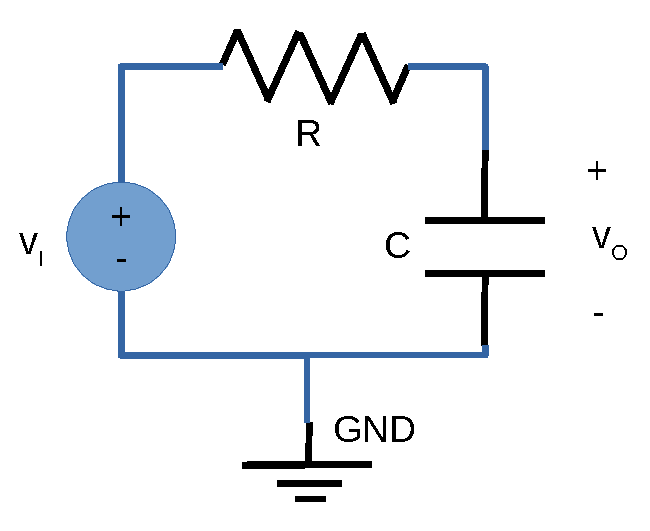
\includegraphics[width=0.4\linewidth]{rc.pdf}
\caption{Voltage driven serial RC circuit.}
\label{fig:rc}
\end{figure}



\section{Theoretical Analysis}
\label{sec:analysis}

In this section, the circuit shown in Figure~\ref{fig:t1} is analysed
theoretically, using the mesh method and the nodal method.

\subsection{Mesh Analysis}
The circuit was analyzed using the 4 elemental meshes, as shown in Figure~\ref{fig:mesh}

\begin{figure}[ht!]
  \centering
  \includegraphics[width=0.4\textwidth]{t1-mesh.pdf}
  \caption{Currents through the elemental meshes.}
  \label{fig:mesh}
\end{figure}

Resulting in the following equations:

\begin{equation}\label{meshEq}
  \begin{cases}
    -R_3(-I_A + I_B) - R_1(-I_A) + V_a + R_4(I_A-I_C) = 0 \\
    I_B = I_b\quad (by\ observation) \\
    -V_c - R_4(-I_C + I_A) + R_6I_C+ R_7I_C = 0 \\
    I_D = I_d\quad (by\ observation) \\
    I_b = K_bV_b = K_bR_3(-I_A + I_B) \\
    V_C = K_CI_C \\
  \end{cases}
\end{equation}

Simplifying in the next matrix system:

\begin{equation}\label{meshM}
  \begin{bmatrix}
    R_3+R_1+R_4 & -R_3 & -R_4 & 0 \\
    K_bR_3 & 1-K_bR_3 & 0 & 0 \\
    -R_4 & 0 & -K_C + R_4+R_6+R_7 & 0 \\
    0 & 0 & 0 & 1\\
  \end{bmatrix}
  \begin{bmatrix}
    I_A\\
    I_B\\
    I_C\\
    I_D\\
  \end{bmatrix}
  =
  \begin{bmatrix}
    -V_a\\
    0\\
    0\\
    I_d\\
  \end{bmatrix}
\end{equation}

Solving the system~\ref{meshM} results in the values in the Table~\ref{tab:mesh}.

\begin{table}[ht!]
  \centering
  \input{../mat/tabmesh.tex}
  \caption{Currents of each mesh.}
  \label{tab:mesh}
\end{table}
\FloatBarrier






\subsection{Nodal Analysis}
The circuit was analyzed using 7 nodes and the GND node, as shown in Figure~\ref{fig:node}

\begin{figure}[ht!]
  \centering
  \includegraphics[width=0.4\textwidth]{t1-node.pdf}
  \caption{Voltage in each node.}
  \label{fig:node}
\end{figure}

Resulting in the following equations:

\begin{equation}\label{nodeEq}
  \begin{cases}
    KCL\ equations:\\
    node\ 2\to (V_1-V_2)G_1 - (V_2-V_3)G_2 - (V_2-V_4)G_3 = 0\\
    node\ 3\to (V_2-V_3)G_2 + I_b = 0\\
    node\ 4\to (V_2-V_4)G_3 + (-V_4)G_4 - (V_4-V_5)G_5 - I_{V_C} = 0\\
    node\ 5\to (V_4-V_5)G_5 + I_d - I_b = 0\\
    node\ 6\to (-V_6)G_6 - (V_6-V_7)G_7 = 0\\
    \\
    Additional\ equations:\\
    V_1 = V_a\\
    I_b = K_b(V_2-V_4)\\
    I_{V_C} = I_d - (V_6-V_7)G_7\\
  \end{cases}
\end{equation}

Simplifying in the next matrix system:

\begin{equation}\label{nodeM}
  \begin{bmatrix}
    1 & 0 & 0 & 0 & 0 & 0 & 0 \\
    G_1 & -G_1-G_2-G_3 & G_2 & G_3 & 0 & 0 & 0 \\
    0 & K_b+G_2 & -G_2 & -K_b & 0 & 0 & 0 \\
    0 & G_3 & 0 & -G_3-G_4-G_5 & G_5 & G_7 & -G_7 \\
    0 & -K_b & 0 & G_5+K_b & -G_5 & 0 & 0 \\
    0 & 0 & 0 & 0 & 0 & -G_6-G_7 & G_7 \\
    0 & 0 & 0 & 1 & 0 & K_cG_6 & -1 \\
  \end{bmatrix}
  \begin{bmatrix}
    V_1\\
    V_2\\
    V_3\\
    V_4\\
    V_5\\
    V_6\\
    V_7\\
  \end{bmatrix}
  =
  \begin{bmatrix}
    V_a\\
    0\\
    0\\
    I_d\\
    -I_d\\
    0\\
    0\\
  \end{bmatrix}
\end{equation}

Solving the system~\ref{nodeM} results in the values in the Table~\ref{tab:node}.

\begin{table}[ht!]
  \centering
  \input{../mat/tabnode.tex}
  \caption{Voltage in each node.}
  \label{tab:node}
\end{table}
\FloatBarrier



\subsection{Results of both methods}
The voltage drop and currents of each resistor were the same of both methods and are shown in the Table~\ref{tab:IeV}.

\begin{table}[ht!]
  \centering
  \input{../mat/tabIeV.tex}
  \caption{Voltage drop and Currents of each resistor.}
  \label{tab:IeV}
\end{table}
\FloatBarrier


%\clearpage
\section{Simulation Analysis}
\label{sec:simulation}

\subsection{Step 1}

Table~\ref{tab:op1} shows the simulated operating point results for the circuit
under analysis, for $t<0$. 


\subsection{Step 2}

Table~\ref{tab:op2} shows the simulated operating point results for the circuit
under analysis, for $t=0$. 

Here, $I_x = -vx\#branch$ because it is not possible to define the current through the voltage source $V_x$ as going from the node n- to the node n+. It may seems that there is current through all the branches and voltages in most of the nodes, but, after observing and considering that the values given by the ``datagen'' file, they have precision till $10^{-11}$, therefore it is possible to say that voltages lesser $10^{-11} V$ and currents lesser than $10^{-11} A$ are indistinguishable from 0.\\


\begin{minipage}[b]{0.46\textwidth}
\centering
   \begin{tabular}{|l|r|}
    \hline    
    {\bf Name} & {\bf Value [A or V]} \\ \hline
    \input{../sim/op1_tab}
   \end{tabular}
    \captionsetup{type=table}   
  \caption{Operating point. A variable preceded by @ or has \# in its name is of type {\em current}
    and expressed in Ampere; other variables are of type {\it voltage} and expressed in
    Volt.}
  \label{tab:op1}
\end{minipage}
\hfill
\begin{minipage}[b]{0.46\textwidth}
\centering
  \begin{tabular}{|l|r|}
    \hline    
    {\bf Name} & {\bf Value [A or V]} \\ \hline
    \input{../sim/op2_tab}
  \end{tabular}
    \captionsetup{type=table}   
  \caption{Operating point. A variable preceded by @ or has \# in its name is of type {\em current}
    and expressed in Ampere; other variables are of type {\it voltage} and expressed in
    Volt.}
  \label{tab:op2}
\end{minipage}


%\clearpage
\subsection{Step 3}

Using as initial condition $V_s=0V$ and $V_c = V_6-V_8$, it was possible to simulate the natural response in the node 6, $v_{6n}(t)$. The plot can be seen in Figure~\ref{fig:sim-v6n}, for $t\in [0,20]ms$.

\begin{figure}[ht!]
    \centering
    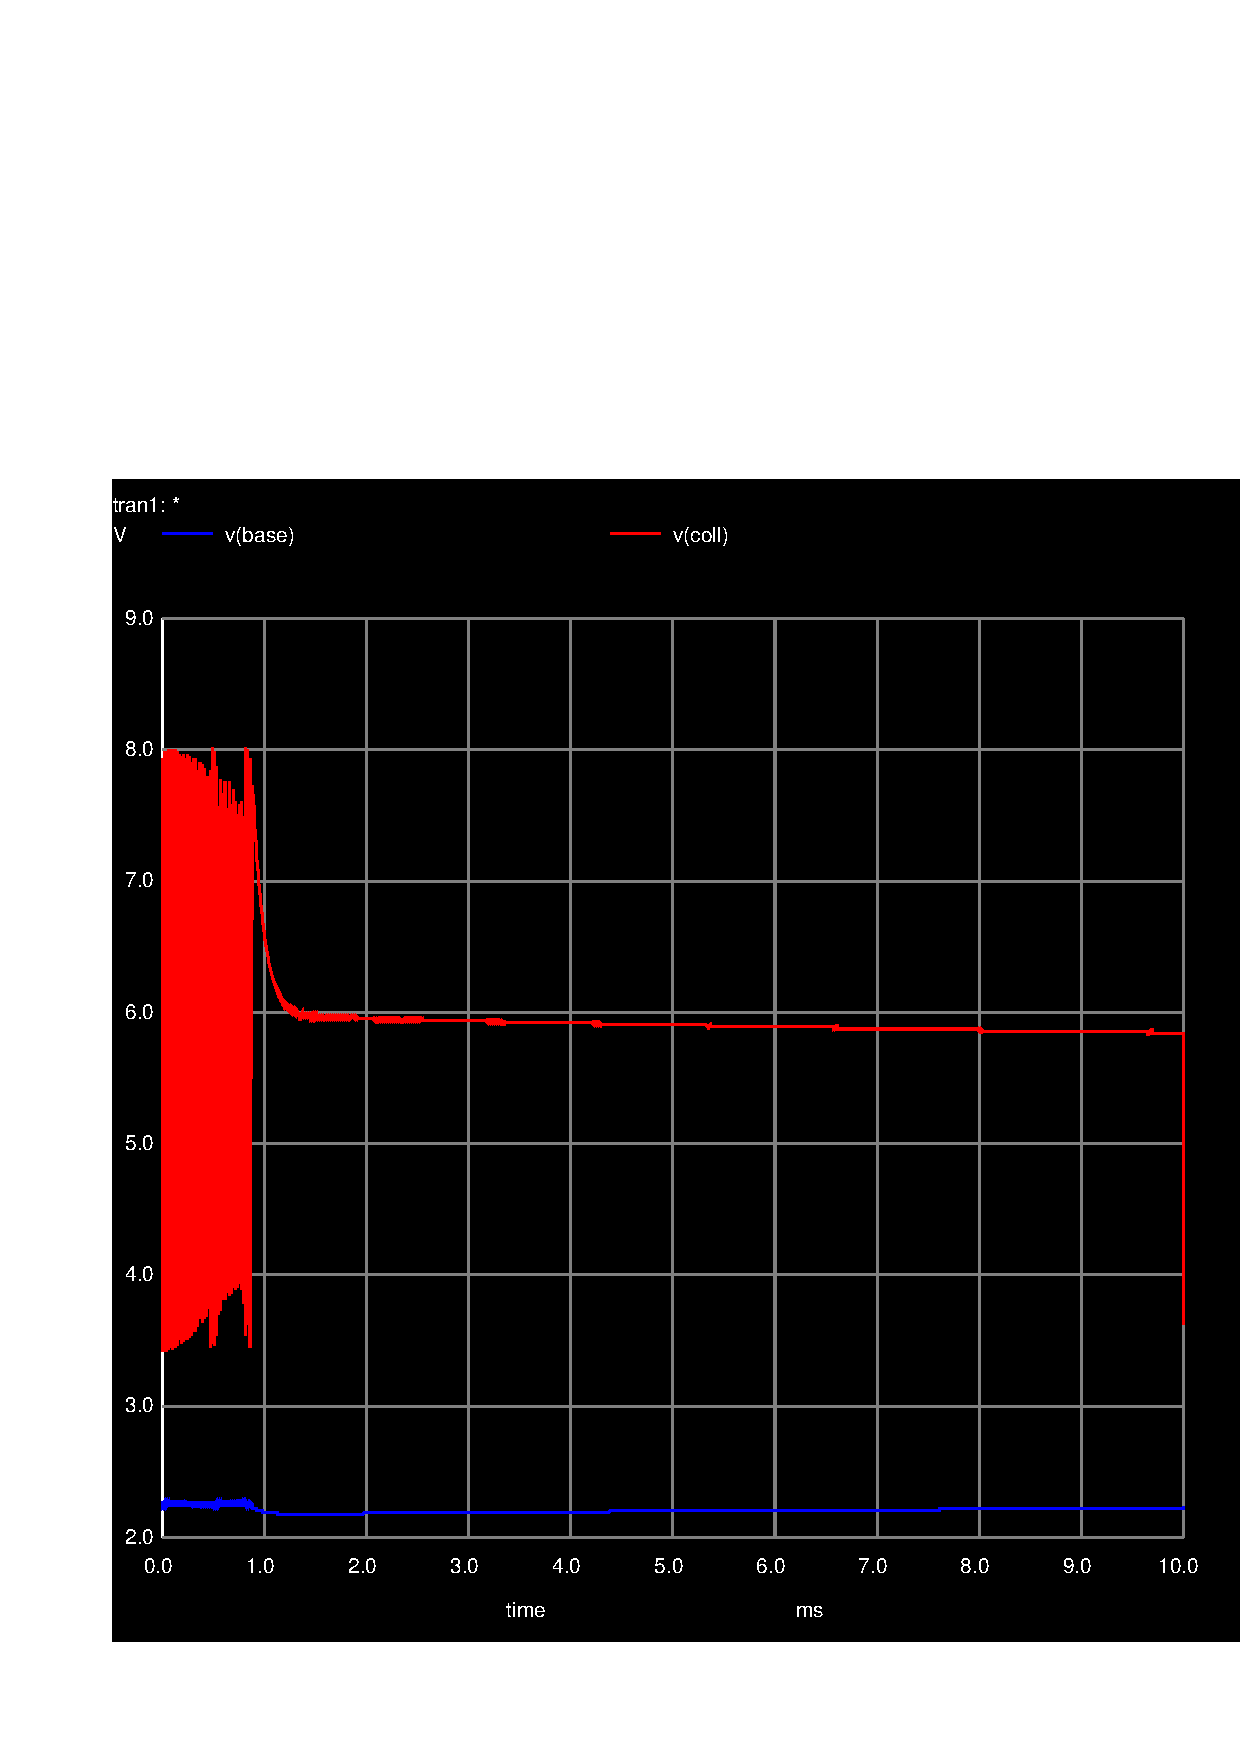
\includegraphics[width=0.5\textwidth, trim={1.8cm 2cm 0 8.1cm}]{../sim/trans.pdf}
    \caption{Natural response in node 6, for $t\in [0,20]ms$.}
    \label{fig:sim-v6n}
\end{figure}
\FloatBarrier




\subsection{Step 4}
Repeating the previous step to simulate the total response on node 6, considering $v_s(t)=~\sin(2 \pi f t)$ and frequency $f=1 kHz$. The plot containing the stimulus and the response can be seen in Figure~\ref{fig:sim-v6total}.

\begin{figure}[ht!]
    \centering
    \includegraphics[width=0.5\textwidth, trim={1.8cm 2cm 0 8.1cm}]{../sim/acdc.pdf}
    \caption{Total response in node 6, for $t\in [0,20]ms$ and $f=1 kHz$.}
    \label{fig:sim-v6total}
\end{figure}
\FloatBarrier



\subsection{Step 5}

\subsubsection{Magnitude Response}

Figure~\ref{fig:sim-db} shows the magnitude of the frequency response for the
circuit under analysis, for the voltages $v_c(f),\ v_6(f)$ and $v_s(f)$, with $f$ from 0.1 \textit{Hz} to 1 \textit{MHz}.

\begin{figure}[ht!] \centering
\includegraphics[width=0.5\linewidth, trim={1.8cm 2cm 0 8.1cm}]{../sim/sim-db.pdf}
\caption{Magnitude response.}
\label{fig:sim-db}
\end{figure}
\FloatBarrier


\subsubsection{Phase Response}

Figure~\ref{fig:sim-phase} shows the phase in degrees of the frequency response for the
circuit under analysis.

\begin{figure}[ht!] \centering
\includegraphics[width=0.5\linewidth, trim={1.8cm 2cm 0 8.1cm}]{sim-phase.pdf}
\caption{Phase response.}
\label{fig:sim-phase}
\end{figure}
\FloatBarrier


\section{Conclusion}
\label{sec:conclusion}

In this laboratory assignment the objective of analysing an RC circuit has been
achieved. Static, time and frequency analyses have been performed both
theoretically using the Octave maths tool and by circuit simulation using the
Ngspice tool. The simulation results matched the theoretical results
precisely. The reason for this perfect match is the fact that this is a
straightforward circuit containing only linear components, so the theoretical
and simulation models cannot differ. For more complex components, the
theoretical and simulation models could differ but this is not the case in this
work.

\lipsum[1-1]

%\cleardoublepage

% ----------------------------------------------------------------------
%  Bibliography
% ----------------------------------------------------------------------
%\addcontentsline{toc}{section}{\bibname}
%\bibliographystyle{abbrvunsrtnat} % <<<<< SELECT IF USING REFERENCES BY NUMBER (CITATION ORDER)
%\bibliography{../../../BIBfile.bib}

% ----------------------------------------------------------------------
\end{document}
% ----------------------------------------------------------------------

